\documentclass[a4paper, 12pt, oneside]{book}
% \documentclass[a4paper, 11pt, oneside]{book}

\usepackage[
    top=25mm,
    bottom=25mm,
    right=25mm,
    left=30mm,
    marginparwidth=10pt,
    marginparsep=15pt
]{geometry}


% \usepackage{natbib}
\usepackage[nottoc]{tocbibind}
\usepackage{microtype}

\usepackage[english]{babel}
\usepackage{blindtext}

\usepackage{amsmath}
\usepackage{amssymb}
\usepackage{amsthm}
\usepackage{siunitx}
% \usepackage{relsize}
\usepackage{cancel}
\usepackage{mathtools}

\usepackage[utf8]{inputenc}
\usepackage[T1]{fontenc}
% \usepackage[notextcomp]{stix2}
% \usepackage{charter}
\usepackage{tgtermes}
\renewcommand{\sfdefault}{ptm}
% \usepackage{stix2}
% \usepackage[scaled=0.865]{helvet}

\usepackage[export]{adjustbox}
\usepackage{graphicx}
\usepackage{tabularx}
\usepackage[svgnames, table]{xcolor}
\usepackage{longtable}
\usepackage[explicit,newparttoc]{titlesec}
\usepackage{titletoc}
\usepackage{etoolbox}
\usepackage{adjustbox}
\usepackage{enumitem}
\usepackage{float}
\usepackage{booktabs, multicol, multirow}
\renewcommand{\aboverulesep}{0pt}
\renewcommand{\belowrulesep}{0pt}
\renewcommand{\arraystretch}{1.2}
% \setlength\cellspacetoplimit{5pt}
% \setlength\cellspacebottomlimit{5pt}


\usepackage{array}
\newcommand{\PreserveBackslash}[1]{\let\temp=\\#1\let\\=\temp}
\newcolumntype{C}[1]{>{\PreserveBackslash\centering}p{#1}}
\newcolumntype{R}[1]{>{\PreserveBackslash\raggedleft}p{#1}}
\newcolumntype{L}[1]{>{\PreserveBackslash\raggedright}p{#1}}

\usepackage{fancyhdr}

\usepackage{mdframed}
\usepackage{tikz}
\usetikzlibrary{positioning}
\usepackage{lastpage}

\usepackage{marginfix}
\usepackage{marginnote}
\usepackage{chngcntr}


\usepackage{hyperref}
\hypersetup{
    colorlinks,
	breaklinks,
	linktocpage=true,
    citecolor=blue,
    filecolor=blue,
    linkcolor=blue,
    urlcolor=blue
}
\usepackage[noabbrev]{cleveref}

% \usepackage[toc,page]{appendix}
\usepackage[toc,page,titletoc,title]{appendix}
\usepackage{bookmark}

\usepackage{xpatch}
\usepackage{ifthen}

\usepackage{imakeidx}
\usepackage[toc,acronym,section]{glossaries}
\usepackage[
	labelfont={color=black,bf,sf},
    % singlelinecheck=false
]{caption}
\usepackage{hhline}

\usepackage{changepage}                 % adjust margins for selected portions
\usepackage{lipsum}

% wide page for side by side figures, tables, etc
\newlength{\offsetpage}
\setlength{\offsetpage}{2.0cm}
\newenvironment{widepage}{\begin{adjustwidth}{-\offsetpage}{-\offsetpage}%
    \addtolength{\textwidth}{2\offsetpage}}%
{\end{adjustwidth}}
% for note
% \newcommand{\handnote}[1]{\sidenote{\footnotesize#1}}
\newcommand{\note}[1]{\marginpar{\footnotesize\fontfamily{cmss}\selectfont#1}}
\renewcommand{\thefootnote}{\arabic{footnote}}

% indexed note
\newcommand{\Note}[3]{\note{\vspace{#3}{#1}}\index{#2}}

% eqauation
\DeclareMathAlphabet{\mathbfsf}{\encodingdefault}{\sfdefault}{bx}{n}
% \renewcommand{\vec}[1]{\mathbfsf{#1}}
\newcommand{\vect}[1]{\vec{\mathbf{#1}}}
\newcommand{\vectwv}[1]{\tilde{\mathbf{#1}}}
\newcommand{\brak}[1]{\langle{#1}\rangle}
\newcommand{\rbrak}[1]{\left({#1}\right)}
\newcommand{\sbrak}[1]{\left[{#1}\right]}
\newcommand{\cbrak}[1]{\left\{{#1}\right\}}
\newcommand{\abrak}[1]{\left|{#1}\right|}
\newcommand{\intInf}{\int_{-\infty}^{+\infty}}
\newcommand{\intinf}{\int_{-\infty}^{\infty}}
\newcommand{\conj}{\mathlarger{*}}%
\newcommand{\Psiconj}{\Psi^\conj}
\newcommand{\Psixt}{\Psi\rbrak{x,t}}
\newcommand{\hi}{\hat{i}}
\newcommand{\hj}{\hat{j}}
\newcommand{\hk}{\hat{k}}
\newcommand{\hx}{\hat{x}}
\newcommand{\hy}{\hat{y}}
\newcommand{\hz}{\hat{z}}
\newcommand{\hr}{\mathbf{\hat{r}}}
\newcommand{\hbx}{\mathbf{\hat{x}}}
\newcommand{\hby}{\mathbf{\hat{y}}}
\newcommand{\hbz}{\mathbf{\hat{z}}}
\newcommand{\hbk}{\mathbf{\hat{k}}}
\newcommand{\vB}{\vect{B}}
\newcommand{\vE}{\vect{E}}
\newcommand{\vD}{\vect{D}}
\newcommand{\vH}{\vect{H}}
\newcommand{\vk}{\vect{k}}
\newcommand{\vr}{\vect{r}}
\newcommand{\vl}{\vect{l}}
\newcommand{\tB}{\tilde{B}}
\newcommand{\tE}{\tilde{E}}
\newcommand{\tD}{\tilde{D}}
\newcommand{\tH}{\tilde{H}}
\newcommand{\curl}[1]{\vect{\nabla}\times\vect{#1}}
\newcommand{\divg}[1]{\vect{\nabla}\cdot\vect{#1}}

% for label 
\newcommand{\labch}[1]{\label{ch:#1}}
\newcommand{\labsec}[1]{\label{sec:#1}}
\newcommand{\labsubsec}[1]{\label{subsec:#1}}
\newcommand{\labequ}[1]{\label{eq:#1}}
\newcommand{\labfig}[1]{\label{fig:#1}}
\newcommand{\labtab}[1]{\label{tbl:#1}}
% and ref
\newcommand{\refch}[1]{\cref{ch:#1}}
\newcommand{\refsec}[1]{\cref{sec:#1}}
\newcommand{\refsubsec}[1]{\cref{subsec:#1}}
\newcommand{\refequ}[1]{\cref{eq:#1}}
\newcommand{\reffig}[1]{\cref{fig:#1}}
\newcommand{\reftab}[1]{\cref{tbl:#1}}
% for Capital first letter ref
\newcommand{\Refch}[1]{\Cref{ch:#1}}
\newcommand{\Refsec}[1]{\Cref{sec:#1}}
\newcommand{\Refsubsec}[1]{\Cref{subsec:#1}}
\newcommand{\Refequ}[1]{\Cref{eq:#1}}
\newcommand{\Reffig}[1]{\Cref{fig:#1}}
\newcommand{\Reftab}[1]{\Cref{tbl:#1}}

% link
\newcommand{\tautkan}{\protect\hyperlink}

% quote
\newcommand{\q}[1]{``#1''}

% new rule
\newcommand{\doublerule}[1][.4pt]{%
	\noindent
	\makebox[0pt][l]{\rule[1.0ex]{\linewidth}{#1}}%
	\rule[.0ex]{\linewidth}{#1}
	\vspace{-0.5cm}
}
\newcommand{\singlerule}[1][.4pt]{%
	\noindent
	\makebox[0pt][l]{\rule[.0ex]{\linewidth}{#1}}%
	\rule[.0ex]{\linewidth}{0pt}
	\vspace{0em}
}

% etc
\newcommand{\autodot}{.}
\newcommand*{\plogo}{\fbox{$\mathcal{PL}$}}

% \renewcommand{\labelitemi}{\tiny$\blacktriangleright$}
% \renewcommand{\labelitemii}{\textbullet}




% Title Page style
\makeatletter
\renewcommand{\maketitle}{
    \bgroup\setlength{\parindent}{0pt}
    \begin{flushleft}
      {\Huge\sffamily\bfseries\@title}
      \vskip 1.5em
      {\sffamily\@author}
      {\sffamily\@date}
    \end{flushleft}\egroup
}
\makeatother


\setlist[itemize]{noitemsep}
\setlist[enumerate]{noitemsep}
\setlist[description]{noitemsep}

% #--------------------------- -----
% Part Style
% #--------------------------- -----
\titleformat{\part}
	[display]
	{\centering\normalfont\Huge\bfseries}
	{\vspace{3pt}\color{black!50}\MakeUppercase{\sffamily{\partname} {\thepart} {#1}}}
	{0pt}
	{\vspace{0.25em}\color{black!20}\titlerule[4pt]\vspace{1pc}}
	\titlespacing*{\part}{0pt}{0pt}{20pt}


% #--------------------------- -----
% Chapter Style
% #--------------------------- -----
% \titleformat{\chapter}
% 	[block]
%     {\bfseries\Huge\sffamily}
%     {\rlap{\hspace*{\dimexpr\linewidth+\marginparsep}
% 		\parbox{\marginparwidth}{\centering\color{black!90}{\Large\MakeUppercase{\so{\chaptername}}}\\[1ex]\color{black!80}\scalebox{4}{\thechapter}}}}
%     {0pt}
%     {\color{black!90}\begin{tabularx}{\linewidth}{@{}>
% 		{\centering\arraybackslash}X>{\centering\arraybackslash}p{1cm}@{\vspace{1.5ex}}}& \makebox[0pt]{\centering}\\[2.5ex] #1\end{tabularx}}
%     [\vspace{0.25em}{\color{black!50}\titlerule[4pt]}\vspace{1.5em}]
% \titlespacing{\chapter}{0pt}{-5ex}{20ex}
\titleformat{\chapter}
	[display]
	{\centering\normalfont\Huge\bfseries}
    {\vspace{3pt}\color{black!90}{\sffamily{\chaptername\ {\thechapter} {#1}}}}
	{0pt}
	{\vspace{0.25em}\color{black!30}\titlerule[2pt]\vspace{1pc}}
	\titlespacing*{\chapter}{0pt}{0pt}{0em}

\titleformat{name=\chapter, numberless}
  [display]
	{\centering\normalfont\Huge\bfseries}
    {\vspace{3pt}\color{black!90}{\sffamily{{} {#1}}}}
	{0pt}
	{\vspace{0.25em}\color{black!30}\titlerule[2pt]\vspace{1pc}}
	\titlespacing*{\chapter}{0pt}{0pt}{0em}

\addto\captionsenglish{\renewcommand{\chaptername}{Bab}}

% #--------------------------- -----
% Section Style
% #--------------------------- -----
% \titleformat{\section}[block]
%   {\large\bfseries}% format applied to label+text
%   {\color{black}\makebox[13pt][r]{\sffamily\thesection\hspace{5pt}\rule{8pt}{8pt}\hspace{5pt}}{\MakeUppercase{\large\sffamily{#1}}}}
%   {0pt}
%   {}% before the title body
%   []% after the title body
% \titleformat{name=\section, numberless}[block]
%   {\large\bfseries}% format applied to label+text
%   {\color{black}\makebox[0cm][r]{\sffamily\thesection\hspace{5pt}\rule{8pt}{8pt}\hspace{5pt}}{\MakeUppercase{\large\sffamily{#1}}}}
%   {0pt}
%   {}% before the title body
%   []% after the title body
% \titleformat{\section}[block]%
%   {\large\bfseries}% format applied to label+text
%   {\color{black!50}\titlerule\vspace{0.5em}\\\color{black}\sffamily\thesection\ {{\large\sffamily{#1}}}}
%   {0pt}
%   {}% before the title body
%   []% after the title body
% \titleformat{name=\section, numberless}[block]
%   {\large\bfseries}% format applied to label+text
%   {\color{black!50}\titlerule\vspace{0.5em}\\\color{black}\sffamily\ {{\large\sffamily{#1}}}}
%   {0pt}
%   {}% before the title body
%   []% after the title body
  
  
% #--------------------------- -----
% Subsection Style
% #--------------------------- -----
% \titleformat{\subsection}%
%   {\normalsize\bfseries}% format applied to label+text
%   {\makebox[0cm][r]{\sffamily\thesubsection\hspace{5pt}\rule{7pt}{7pt}\hspace{5pt}}{\normalsize\sffamily{#1}}}% label
%   {0pt}
%   {}% before the title body
%   []% after the title body
\titleformat{\subsection}%
  {\normalsize\bfseries}% format applied to label+text
  {\sffamily\thesubsection\ {{\normalsize\sffamily{#1}}}}
  {0pt}
  {}% before the title body
  []% after the title body
  
  

% #--------------------------- -----
% Header Style
% #--------------------------- -----
\setlength{\headheight}{14.5pt}
\pagestyle{fancy}
\fancyhead{}\fancyfoot{}
\fancyhead[LO]{\sffamily\small\nouppercase{\leftmark}}
\fancyhead[R]{\sffamily\small\nouppercase{\textit{Oleh: Firman Qashdus Sabil}}}
\fancyfoot[OL]{\thepage}%
\renewcommand{\headrulewidth}{0.5pt}
% for first page
\fancypagestyle{plain}
{
    \setlength{\headheight}{14pt}
    \fancyhf{}%
    \fancyfoot[R]{\sffamily\small{\sffamily\bfseries\thepage}}
    \renewcommand{\headrulewidth}{0pt}
    \renewcommand{\footrulewidth}{0.4pt}
}


% #--------------------------- -----
% Table of Contents, Figures, and Tables
% #--------------------------- -----
% if you want to add doted line between content-name and content page
% change the 4th paremater --> {\contentspage} to this: {\titlerule*[0.6pc]{.}\contentspage}
\setlength{\titlewidth}{0.6\textwidth} % title rule reduced to 0.6 of textwidth instead of full textwidth
\let\oldtitleline\titleline{}
\renewcommand{\titleline}{\oldtitleline*}
\titlecontents{chapter}
  [2.1em]
  {\vspace{1em}\bfseries\large\sffamily}
  {\contentslabel[\thecontentslabel\hspace{0.35em}\rule{0.6em}{0.6em}]{2em}}
  {\hspace{-1.8em}}
  {\hfill\contentspage}
  [\vspace{0.2em}]

\titlecontents{section}
  [4.2em]
  {\sffamily}
  {\contentslabel{2.5em}}
  {\hspace*{0em}}
  {\contentspage}
  [\vspace{0.2em}]

\titlecontents{subsection}
  [7.1em]
  {\sffamily}
  {\contentslabel{2.5em}}
  {\hspace*{0em}}
  {\contentspage}
  [\vspace{0.2em}]

% #--------------------------- -----
% Caption and Ref Name
% #--------------------------- -----
\addto\captionsenglish{\renewcommand{\figurename}{Gambar}}
\addto\captionsenglish{\renewcommand{\tablename}{Tabel}}
\addto\captionsenglish{\renewcommand{\bibname}{Referensi}}
\addto\captionsenglish{\renewcommand{\chaptername}{Bab}}

\crefname{equation}{persamaan}{equations}
\Crefname{equation}{Persamaan}{Equations}
\crefname{table}{tabel}{tables}
\Crefname{table}{Tabel}{Tables}
\crefname{figure}{gambar}{gambar}
\Crefname{figure}{Gambar}{Figures}


% #--------------------------- -----
% Bibliography using natbib
% #--------------------------- -----



% #--------------------------- -----
% Indentation
% #--------------------------- -----
\setlength\parindent{1.5em}


% #--------------------------- -----
% Get rid off underfull badness warning
% Since this usually not clearly look 
% by the eye. 
% (you may want to still show it if 
% really want perfect typset)
% #--------------------------- -----
\hbadness=99999
\vbadness=99999


\renewcommand{\contentsname}{Daftar Isi}
\renewcommand{\listfigurename}{Daftar Gambar}
\renewcommand{\listtablename}{Daftar Tabel}
% problem style theorem
\newtheoremstyle{problemstyle}  %   <name>
        {0pt}                       % <space above>
        {0pt}                       % <space below>
        {\normalfont}               % <body font>
        {}                          % <indent amount}
        {\bfseries}                 % <theorem head font>
        {\normalfont\bfseries}      % <punctuation after theorem head>
        {.5em}                      % <space after theorem head>
        {}                          % <theorem head spec (can be left empty, meaning `normal')>
\theoremstyle{problemstyle}
\newtheorem{problem}{\sffamily Problem}[section]

% Important Equation
\newenvironment{Equation}
    {
        \vspace{0.3em}\begin{mdframed}[
            backgroundcolor=gray!25,
            linecolor=black!90!white,
            linewidth=0.6pt,
            skipabove=0.5em,
            skipbelow=0.5em,
            innertopmargin=0.6em,
            innerbottommargin=0.6em,
            topline=true,
            leftline=true, 
        ]\begin{equation}
    }
    {
        \end{equation}\end{mdframed}
    }

\newenvironment{problembox}{
    \begin{mdframed}[
        backgroundcolor=gray!15!white,
        linecolor=black!90!white,
        linewidth=0.5pt,
        innertopmargin=10pt,
        innerbottommargin=10pt,
        innerleftmargin=5pt,
        innerrightmargin=5pt,
        topline=false,
        leftline=false, 
    ]
}{
    \end{mdframed}
}


% #-------------------------------
%	Uncountered Box
% #-------------------------------
\mdfdefinestyle{fqsboxstyle}{
	skipabove=1.5\topskip,
	skipbelow=.5\topskip,
	rightmargin=0pt,
	leftmargin=0pt,
	%innertopmargin=3pt,
	%innerbottommargin=3pt,
	innerrightmargin=7pt,
	innerleftmargin=7pt,
	topline=false,
	bottomline=false,
	rightline=false,
	leftline=false,
	%linewidth=1pt,
	%roundcorner=0pt,
	%font={},
	%frametitlefont={},
	frametitlerule=true,
	linecolor=black,
	%backgroundcolor=LightBlue,
	fontcolor=black,
	%frametitlebackgroundcolor=LightBlue,
}
\newmdenv[
	style=fqsboxstyle,
	backgroundcolor=RoyalBlue!25!White,
	frametitlebackgroundcolor=RoyalBlue!25!White,
]{fqsbox}

%-------------------------------
%	Countered Box
%-------------------------------
\newcounter{fqscounter}[section]
\newenvironment{fqscounter}[1][]{\refstepcounter{fqscounter}
	\begin{fqsbox}[frametitle=Comment~\thesection\autodot\thefqscounter#1.]
}{
	\end{fqsbox}\vspace{1em}
}

\setlist[itemize]{noitemsep, topsep=0pt, leftmargin=*}
\setlist[enumerate]{noitemsep, topsep=0pt, leftmargin=*}

% \title{LA}
% \author{Firman Qashdus Sabil.}
% \date{\today}
\begin{document}
% \begin{titlepage}
% \thispagestyle{empty}
% \maketitle
% \hrule\vspace{1em}
% \end{titlepage}
% \tableofcontents
\clearpage
\hspace*{-0.26in}
\begin{minipage}{0.3\textwidth}
\flushleft\includegraphics[width=2cm]{gambar/Lambang-UM.png}
\end{minipage}
%% temporary titles
% command to provide stretchy vertical space in proportion
\newcommand\nbvspace[1][3]{\vspace*{\stretch{#1}}}
% allow some slack to avoid under/overfull boxes
\newcommand\nbstretchyspace{\spaceskip0.5em plus 0.25em minus 0.25em}
% To improve spacing on titlepages
\newcommand{\nbtitlestretch}{\spaceskip0.3em}
\pagestyle{empty}
\begin{flushleft}
\bfseries
% \nbvspace[1]
\vspace{6mm}
\Huge
{
	\nbtitlestretch\fontsize{18pt}{18pt}\selectfont PENGUKURAN INTENSITAS CAHAYA MATAHARI DALAM SATU HARI DENGAN MENGGUNAKAN LUX METER
}

\vspace{0.5em}
\normalfont\small Projek I OPTIKA
\vspace{1em}

\normalfont\small Disusun oleh:\\
\normalfont\small Firman Qashdus Sabil (210321606892), Offering: AC\\%[0.5em]
\normalfont\small untuk Memenuhi Tugas Mata Kuliah Optika \\
\normalfont\small yang diampu Dr. Cahyo Aji Hapsoro M.Si

\vspace{15em}\begin{center}
\begin{tikzpicture}[overlay, remember picture, node distance={2pt}, transform canvas={scale=0.9}]
	\node (tapir) {\includegraphics[width=10cm]{gambar/cover_hero.jpg}};
	% \node[black!85, above right=of tapir.north, rotate=5] (fundcalc) {$E(\si{lux})=\frac{\phi(\si{lumen})}{A(\si{m^2})}$};
	% \node[black!70, above left=of fundcalc, rotate=-5] (orth) {$d\vB = \frac{\mu_0 I}{4\pi} \frac{d\vl \times \hr}{r^2}$};
	% \node[black!75, above right=of orth, rotate=-3, xshift=15pt] (diff) {$\mathbf{\nabla}\cdot\mathbf{B}=0$};
	% \node[black!60, right=of diff, rotate=3, yshift=-15pt] (vecdef) {$\mathbf{B}=\frac{\mu_0 I}{2 \pi R}$};
	% \node[black!40, below left=of orth, rotate=-9] (euler) {$\mathbf{\nabla}\times\mathbf{B}=\mu_0 \mathbf{J}+\frac{1}{c^2}\frac{\partial \mathbf{E}}{\partial t}$};
	% \node[black!30, above left=of diff] (eigendecomp) {$\sin{\phi}$};
	% \node[black!90, below right=of fundcalc, xshift=10pt, yshift=15pt, rotate=-10] (taylorcos) {$\bar{b}=\frac{n \sum\left(x y\right)-\sum x \sum y}{n \sum x^2-\left(\sum x\right)^2}$};
	% \node[black!25, above right=of diff, xshift=10pt, yshift=-10pt] (gamma) {$r=\frac{s}{\cos{\alpha}}$};
	% \node[black!20, above=of diff, xshift=-5pt, yshift=15pt, rotate=-7] (lintrans) {$S_a = S_y \sqrt{\frac{\sum x^2}{n\sum x^2 - (\sum x)^2}}\ \text{  dan  }\ S_b = S_y \sqrt{\frac{n}{n\sum x^2 - (\sum x)^2}}$};
	% \node[black!20, above left=of eigendecomp, rotate=-7] (binom) {$R_a =\frac{S_a}{a}$};
	% \node[black!15, above left=of orth, rotate=3] (rot) {$\bar{a}=\frac{\left(\sum y\right)\left(\sum x^2\right)-\left(\sum x\right)\left(\sum x y\right)}{n\left(\sum x^2\right)-\left(\sum x\right)^2}$};
	% \node[black!13, above left=of gamma, yshift=15pt, rotate=5] (expand) {$(a+b)^{n}=\sum\limits_{k=0}^{n}\binom{n}{k}a^{n-k}b^{k}$};
	% \node[black!10, above left=of binom, rotate=3] (elog) {$a^{b}=\eu^{b\log(a)}$};
\end{tikzpicture}\end{center}
\nbvspace[3]
\normalsize

\large

\vspace{2em}
\fontsize{13pt}{13pt}\bfseries\sffamily\selectfont UNIVERSITAS NEGERI MALANG\\\vspace{0.2cm}
\fontsize{13pt}{13pt}\bfseries\sffamily\selectfont FAKULTAS MATEMATIKA DAN ILMU PENGETAHUAN ALAM\\\vspace{0.2cm}
\fontsize{13pt}{13pt}\bfseries\sffamily\selectfont PROGRAM STUDI PENDIDIKAN FISIKA\\\vspace{0.2cm}
\fontsize{13pt}{13pt}\bfseries\sffamily\selectfont DESEMBER 2023




\end{flushleft}
\newpage
\pagestyle{fancy} % otherwise fancy headers disappear

\tableofcontents
\listoftables
\listoffigures

\newpage
% BEGIN DOCUMENTS
% >>>>>>>>>>>>>>>>>>> CHAPTER 1 PENDAHULUAN
\chapter{Pendahuluan}
\section{Latar Belakang}
Matahari, sebagai bintang pusat tata surya, menyediakan sumber energi utama bagi kehidupan di Bumi. Dari Bumi, matahari berjarak sekitar 150 juta kilometer. Energi matahari diterima oleh Bumi dalam bentuk radiasi elektromagnetik \cite{blal2020prediction}. Radiasi elektromagnetik ini mencakup berbagai panjang gelombang, termasuk cahaya tampak \cite{rokhaniyah2019alat}. Cahaya matahari adalah pendorong utama semua proses atmosfer, iklim, serta merupakan kunci bagi kelangsungan hidup ekosistem di Bumi \cite{hader2007effects,zarnetske2021potential}. Seiring perputaran Bumi pada sumbunya, terjadi perubahan siklus siang dan malam yang menciptakan variasi harian dalam intensitas cahaya matahari. 

Intensitas cahaya matahari yang bervariasi dapat mempengaruhi suhu udara di berbagai lokasi geografis di Bumi. Suhu udara dapat terpengaruh karena seluruh energi dari matahari, sampai ke Bumi dalam bentuk radiasi matahari \cite{wald:hal-01676634}. Radiasi ini merupakan salah satu cara untuk mendistribusikan panas. Inilah yang mengakibatkan intensitas cahaya matahari berpengaruh terhadap suhu udara yang dilewatinya. Energi panas dari sinar matahari diserap oleh partikel-partikel udara, benda, dan permukaan bumi \cite{Lipinski2021-lp}. Pemanasan yang disebabkan oleh paparan langsung matahari dapat meningkatkan suhu di siang hari, sementara kurangnya radiasi matahari pada malam hari dapat menyebabkan penurunan suhu. Selain suhu, intensitas cahaya matahari juga mempengaruhi kelembapan udara. Proses penguapan yang ditingkatkan oleh sinar matahari dapat meningkatkan kelembapan udara di sekitarnya. 

Oleh karena itu, dilakukan percobaan pengukuran intensitas cahaya matahari tiap jam selama 24 jam. Untuk mengukur intensitas cahaya matahari tiap jamnya digunakan perangkat \textit{smartphone} yang memiliki sensor cahaya dengan aplikasi \textit{Pengukur Cahaya}. Besarnya intensitas cahaya matahari perlu diukur karen pada dasarnya segala aktivitas dan teknologi energi terbarukan banyak memanfaatkan matahari sebai sumber energi utamanya.
\section{Tujuan}
Adapun tujuan dilakukannya percobaan ini adalah:
\begin{enumerate}
    \item Mengetahui bagaimana hubungan antara waktu pengukuran terhadap hasil pengukuran intensitas cahaya matahari.
    \item Mengetahui bagaimana hubungan antara posisi matahari dari titik pengukuran terhadap hasil pengukuran intensitas cahaya matahari
    \item Mengetahui pengaruh intensitas cahaya matahari terhadap suhu udara di area pengukuran.
    \item Mengetahui pengaruh intensitas cahaya matahari terhadap kelembapan udara di area pengukuran.
\end{enumerate}
\section{Manfaat}
Manfaat yang diperoleh dari percobaan ini adalah
\begin{enumerate}
    \item Memperoleh pemahaman terkait intensitas cahaya matahari
    \item Memperoleh pemahaman terkait besaran-besaran yang mempengaruhi hasil pengukuran intensitas cahaya matahari
    \item Memperoleh pemahaman terkait pengaruh intensitas cahaya matahari terhadap suhu udara.
    \item Memperoleh pemahaman terkait pengaruh intensitas cahaya matahari terhadap kelembapan udara.
\end{enumerate}

% >>>>>>>>>>>>>>>>>>> CHAPTER 2 DASAR TEORI
\chapter{Dasar Teori}
\section{Cahaya}
Sebelum permulaan abad ke-19, cahaya dianggap sebagai sebuah aliran partikel yang dipancarkan oleh suatu sumber yang dilihat oleh mata \cite{Serway2018-if}. Newton sebagai arsitek utama model partikel dari cahaya, berpendapat bahwa partikel dipancarkan dari sumber cahaya dan partikel ini merangsang indra penglihatan saat memasuki mata \cite{Serway2018-if}. Dengan menggunakan ide ini, dia mampu menjelaskan pemantulan dan pembiasan. Sebaliknya Christian Huygens menunjukkan bahwa model gelombang dari cahaya juga dapat menjelaskan pemantulan dan pembiasan \cite{Pedrotti2006-ek}. Sifat cahaya sebagai gelombang diperkuat dengan eksperimen interferensi cahaya yang dilakukan Thomas Young dan hasil kerja Maxwell yang menunjukkan bahwa cahaya adalah bentuk dari gelombang elektromagnet dengan frekuensi tinggi \cite{Hecht2015-by}.

Model cahaya sebagai gelombang dan teori elektromagnet klasik mampu menjelaskan berbagai sifat cahaya, tetapi terdapat beberapa hasil eksperimen yang tidak dapat dijelaskan dengan model ini, misalnya efek fotolistrik \cite{Hecht2015-by}. Einstein mengusulkan penjelasan dari efek fotolistrik menggunakan pemodelan berdasarkan kuantisasi yang dikembangkan Max Planck \cite{Krane2012-fm}. Model kuantisasi cahaya ini menyatakan bahwa energi dari sebuah gelombang cahaya ada dalam sebuah partikel foton \cite{Krane2012-fm}. Cahaya merambat dalam ruang vakum dengan kecepatan $3\times 10^8\ \si{m/s}$

\section{Cahaya Matahari}
\subsection{Radiasi Cahaya Matahari}
Radiasi matahari merupakan gelombang elektromagnetik dengan komponen medan listrik $\vec{E}$ dan medan magnet $\vec{B}$ \cite{Hecht2015-by}. Radiasi cahaya matahari yang mengenai Bumi disebut insolasi. Intensitas radiasi sinar matahari berkurang sebesar $1/R^2$ jarak dari matahari.
\subsection{Intensitas Cahaya Matahari}
Intensitas adalah besaran daya yang dipancarkan oleh cahaya persatuan luas. Satuan dari intensitas cahaya adalah Candela (CD). Alat yang digunakan untuk mengukur intensitas cahaya adalah luxmeter. 

\section{Pengukuran Cahaya Matahari}
\subsection{Istilah dan Besaran yang Diukur Pada Pengukuran Cahaya Matahari}
Beberapa istilah yang perlu diketahui dalam pengukuran intensitas cahaya matahari adalah
\begin{description}
    \item[Luminous Flux] berasal dari bahasa latin \q{Fluxus} yang artinya aliran. Dalam hal cahaya, luminous flux diartikan sebagai arus cahaya $\Pi$ yang dipancarkan tiap waktu. Luminous Flux memiliki satuan Lumen(lm).
    \item[Illuminan] Adalah banyaknya luminous flux tiap satuan luas. Illuminan memiliki satuan Lux
    \item[Intensitas Cahaya] adalah besarnya cahaya tampak yang dipancarkan dalam satuan waktu untuk tiap sudut ruang. Satuan dari intensitas cahaya adalah Candela.
\end{description}

\subsection{Sudut Datang atau Altitude dari Sinar Matahari}
Sudut datang dari sinar matahari adalah sudut yang terbentuk antara sinar datang matahari terhadap permukaan bumi. Saat matahari tepat berada di suatu titik (membentuk sudut datang $90^\circ$) maka penyinaran matahari terjadi secara maksimal sehingga suhunya juga maksimal. Sedangkan pada sudut datang kurang atau lebih dari $90^\circ$ maka penyinaran matahari semakin berkurang. Semakin besar sudut datang sinar matahari maka sinar tersebut akan terproyeksi pada satuan yang lebih sempit, sehingga energi tiap satuan luas yang diterima semakin besar. Selain itu, semakin besar sudut datang sinar matahari maka semakin pendek lintasan atmosfer yang dilalui sinar \cite{herreria2020solar}. Penggambaran sudut altitude dapat dilihat pada \reffig{azimuthx}.
\subsection{Letak Lintang dari Titik Pengukuran Cahaya Matahari}
Bentuk bulat dari Bumi mengakibatkan variasi perolehan cahaya matahari di tempat yang berbeda. Salah satu garis pembagi bumi adalah garis lintang. Garis lintang adalah garis imajiner yang membentang dari timur ke barat di sepanjang permukaan Bumi dan diukur dalam derajat terhadap garis khatulistiwa. Garis lintang diukur dari $0^\circ$ (khatulistiwa) hingga maksimal $90^\circ$ di utaran atau selatan. Daerah dengan lintang $0^\circ$ lebih dekat dengan matahari sehingga menerima cahaya matahari lebih banyk dibandingkan dengan daerah pada lintang $90^\circ$. Dalam percobaan ini, titik pengukuran terletak pada garis lintang $-8,0904651^\circ$.

\subsection{Sudut Azimuth Matahari dari Titik Pengukuran Cahaya Matahari}
Sudut azimuth seperti kompas yang menunjukkan arah terbitnya matahari. Pada siang hari untuk belahan Bumi bagian utara matahari selalu tepat berada di sebelah selatan dan sebaliknya untuk belahan bumi bagian selatan. Penggambaran sudut azimuth dapat dilihat pada \reffig{azimuthx}.
\begin{figure}[H]
    \centering
    \includegraphics[width=0.4\textwidth]{gambar/azimuth.png}
    \caption{Sudut altitude dan azimuth. Sudut azimuth berperan sebagai arah kompas dengan utara $0^\circ$ dan selatan $180^\circ$}
    \labfig{azimuthx}
\end{figure}

\subsection{Sudut Deklinasi Matahari}
Sudut deklinasi yang disimbolkan dengan $\delta$ bervariasi tiap musimnya karena kemiringan bumi pada sumbu rotasinya dan rotasi bumi mengelilingi matahari. Kemiringan bumi terhadap sumbu rotasinya adalah sebesar $\pm 23,45^\circ$
\begin{figure}[H]
    \centering
    \includegraphics[width=0.8\textwidth]{gambar/declination1.png}
    \caption{Sudut deklinasi Bumi tiap musim }
    \labfig{declination 1}
\end{figure}
Deklinasi matahari adalah sudut antara garis khatulistiwa dan garis yang ditarik dari pusat bumi ke pusat matahari.
\begin{figure}[H]
    \centering
    \includegraphics[width=0.8\textwidth]{gambar/declination2.png}
    \caption{Sudut deklinasi matahari}
    \labfig{declination 2}
\end{figure}
Sudut deklinasi dapat dihitung dengan persamaan
\begin{equation*}
    \delta = -23,45^\circ \times \cos\rbrak{\frac{360}{365}\times \rbrak{d+10}},
\end{equation*}
dimana $d$ adalah hari dalam satu tahun, dengan 1 Januari sebagai $d=1$.
% \subsection{Kejernihan Atmosfer}
% text

\section{Hubungan Suhu dengan Kelembapan}
Kemampuan udara untuk mempertahankan uap air bergantung pada suhunya. Dengan adanya perubahan suhu udara, kemampuan mempertahankan kelembapan dapat meningkat atau menurun, sehingga memengaruhi kelembapan relatif. Hubungan antara kelembaban dan suhu berbanding terbalik. Jika suhu meningkat, maka kelembaban relatif akan berkurang, dengan demikian udara akan menjadi lebih kering. Saat suhu menurun, udara akan menjadi lebih basah, oleh karena itu kelembaban relatif akan meningkat \cite{widhiada2019robust}.

\section{Instrumen Pengukuran Intensitas Cahaya Matahari Berbasis Android}
Selama beberapa tahun terakhir, \textit{smartphone} berbasis Android atau iPhone dianggap sebagai ponsel multifungsi yang canggih. Dalam kasus Android, biasanya terdapat setidaknya empat sensor berbeda yang memungkinkan pengguna memantau beberapa besaran seperti kelembapan, pencahayaan, tekanan, dan suhu sekitar. Sensor cahaya misalnya, digunakan oleh \textit{smartphone} untuk mengatur pencahayaan layar secara otomatis \cite{esmaeili2019mobile}. Sebagai contoh pada ruangan yang terang, maka kecerahan layar \textit{smartphone} akan meningkat agar dapat tetap dibaca oleh pengguna dangan baik. Sebaliknya pada ruangan yang gelap kecerahan layar \textit{smartphone} akan menurun agar mata pengguna tidak kelelahan. Sensor cahaya pada smartphone mampu menghasilkan pengukuran yang akurat. Namun, secara teoritis, sensor tersebut tidak dapat dibandingkan dengan keakuratan perangkat keras khusus yang memang di desain untuk mengukur intensitas cahaya matahari.

Dalam rangka menghubungkan \textit{hardware} sensor cahaya dengan antarmuka pengguna maka diperlukan sebuah \textit{software} pengukur cahaya. Pada sistem operasi Android, terdapat banyak pilihan aplikasi sensor cahaya yang dapat digunakan. Pada projek ini nama aplikasi yang digunakan adalah \textit{Pengukur Caaya} sebagaimana pada bagian langkah percobaan.

\section{Database Cuaca}
Database cuaca disini maksudnya adalah media-media yang menyimpan histori cuaca berupa temperatur, prediksi hujan, kelembapan, dan parameter-parameter cuaca lainnya. Salah satu penyedia histori cuaca adalah \href{https://www.visualcrossing.com/about}{visualcrossing.com}. Platform ini menyediakan histori laporan cuaca dalam bentuk data cuaca dan \textit{application programming interface} (API).
\begin{figure}[H]
    \centering
    \includegraphics[width=0.8\textwidth]{gambar/Langkah/vc1.png}
    \caption{Platform penyedia histori laporan cuaca \href{https://www.visualcrossing.com/about}{visualcrossing.com}}
\end{figure}

\section{Instrumen Perhitungan Posisi Matahari Berbasis Web}
Aplikasi web \href{https://www.suncalc.org/#/-8.0905,112.6468,18/2023.11.10/18:00/1/3}{suncalc} digunakan untuk melakukan perhitungan posisi matahari. Data posisi matahari yang bisa didapat dari aplikasi web ini berupa data altitude, azimuth, deklinasi, dan beberapa data lain. Pengguna dapat menghitung data posisi matari berdasarkan tanggal dan jam yang ditentukan.
\begin{figure}[H]
    \centering
    \includegraphics[width=0.8\textwidth]{gambar/Langkah/vc2.png}
    \caption{Aplikasi perhitungan posisi matahari \href{https://www.suncalc.org}{suncalc}}
\end{figure}

\section{Instrumen Penentuan Letak di Permukaan Bumi (GPS)}
Google maps adalah aplikasi yang dapat digunakan untuk menentukan titik pengambilan data. Untuk dapat menggunakannya, \textit{smartphone} harus memiliki akses internet dan sistem GPS yang aktif.
\begin{figure}[H]
    \centering
    \includegraphics[width=0.8\textwidth]{gambar/Langkah/maps.png}
    \caption{Aplikasi perhitungan posisi pengukuran \href{https://www.google.com/maps}{Google maps}}
\end{figure}


% >>>>>>>>>>>>>>>>>>> CHAPTER 3 PERCOBAAN
\chapter{Metode Percobaan}
\section{Lokasi dan Waktu Percobaan}
\subsection{Lokasi Percobaan}
Lokasi percobaan adalah Jln. Krapyak Jaya, Desa Krebet Senggrong, Kec. Bululawang, Kab. Malang, Jawa Timur, pada koordinat lintang: $-8.0904651^\circ$ dan bujur: $112.6468429^\circ$. Lokasi percobaan adalah persawahan terbuka tanpa adanya objek-objek tinggi yang dapat mengganggu pengukuran data.
\begin{figure}[h]
    \centering
    \includegraphics[width=1\textwidth]{gambar/Dokumentasi/lokasi-percobaan-cropped.pdf}
    \caption{Lokasi percobaan (\href{https://maps.app.goo.gl/vQ3tZS5WpQbmFbkh7}{tautan google maps})}
    \labfig{3-1-lokasi-percobaan}
\end{figure}

\subsection{Waktu Percobaan}
Percobaan dilakukan pada hari Jum'at, 10 November 2023 pukul 19.00 WIB s.d. Sabtu, 11 November 2023 pukul 18.00 WIB. Kondisi cuaca pada tanggal 10 November 2023 pukul 19.00 WIB s.d. Sabtu, 11 November 2023 pukul 14.00 WIB cerah. Sedangkan pada Sabtu, 11 November 2023 pukul 15.00 s.d. 18.00 berawan.


\section{Alat dan Bahan}
Alat dan bahan yang digunakan dalam percobaan ini adalah
\begin{center}
        \setlength\LTleft{-2mm}\begin{longtable}{p{0.2cm}  p{6cm}  p{6cm}}  
            % \toprule
            %%%%%%%% Next ROw %%%%%%%% 
            \text{1.}
            &
            \adjustbox{valign=t}{\includegraphics[width=6cm]{gambar/Dokumentasi/smartphone-complete.pdf}}\vspace{0.5cm}
            &
            \textit{Smartphone} Oppo A17 dengan sensor cahaya dibagian depan, aplikasi jam bawaan, dan aplikasi \textit{Pengukur Cahaya}.\\
             %%%%%%%% Next ROw %%%%%%%% 
            % \cmidrule(r){1-3}
            \text{2.}
            &
            \adjustbox{valign=t}{\includegraphics[width=6cm]{gambar/Dokumentasi/jam-digital-com.pdf}}\vspace{0.5cm}
            &
            Jam digital dari Gawai.\\
            %%%%%%%% Next ROw %%%%%%%% 
            % \cmidrule(r){1-3}
            \text{3.}
            &
            \adjustbox{valign=t}{\includegraphics[width=6cm]{gambar/Dokumentasi/lux-meter-com.pdf}}\vspace{0.5cm}
            &
            Aplikasi \textit{Pengukur Cahaya} untuk mengukur intensitas cahaya matahari.\\
            %%%%%%%% Next ROw %%%%%%%% 
            % \cmidrule(r){1-3}
            \text{4.}
            &
            \adjustbox{valign=t}{\includegraphics[width=6cm]{gambar/Dokumentasi/suncalc-comp.png}}\vspace{0.5cm}
            &
            Aplikasi web \href{https://www.suncalc.org/#/-8.0905,112.6468,17/2023.11.10/18:00/1/3}{suncalc.org} untuk menghitung posisi matahari (derajat azimuth, altitude, dan deklinasi) dari lokasi pengukuran.\\
            % \bottomrule
            %%%%%%%% Next ROw %%%%%%%% 
            % \cmidrule(r){1-3}
            \text{5.}
            &
            \adjustbox{valign=t}{\includegraphics[width=6cm]{gambar/Dokumentasi/visualcrossing.png}}\vspace{0.5cm}
            &
            Aplikasi web histori cuaca \href{https://www.visualcrossing.com/weather-history}{visualcrossing} untuk mendapatkan kondisi cuaca dari lokasi pengukuran.\\
            % \bottomrule
        \end{longtable}
    \label{table:alat-dan-bahan}
\end{center}
\vspace{-3em}
% \section{Skema Percobaan}
% \input{contents/3-3-skema-percobaan.tex}
\section{Variabel Percobaan}
\subsection{Variabel Bebas}
Variabel bebas adalah variabel yang diubah atau dimanipulasi oleh peneliti dalam percobaan. Percobaan dirancang untuk menguji pengaruh variabel bebas terhadap variabel terikat. Variabel bebas dalam penelitian ini adalah posisi matahari, berupa sudut azimuth, altitude, dan deklinasi tiap jam selama 24 jam.
\subsection{Variabel Terikat}
Variabel terikat adalah variabel yang diukur atau diamati sebagai respons terhadap perubahan pada variabel bebas. Variabel terikat dalam percobaan ini adalah besar intensitas cahaya matahari, suhu udara, dan kelembapan udara.
\subsection{Variabel Kontrol}
Variabel kontrol adalah variabel yang tetap konstan atau diatur sedemikian rupa agar tidak berubah selama percobaan. Variabel kontrol membantu memastikan bahwa perubahan yang diamati pada variabel terikat dapat dengan yakin diatribusikan kepada perubahan dari variabel bebas, bukan faktor-faktor lain. Variabel kontrol dalam percobaan ini adalah titik koordinat/lokasi pengambilan data, jenis \textit{smartphone}, \textit{software} penghitung posisi matahari, dan \textit{software} pangukur intensitas cahaya matahari yang digunakan.
\section{Langkah Percobaan}
\subsection{Penentuan Lokasi Pengukuran}
\begin{enumerate}[leftmargin=*, label=\alph*]
    \item Mencari titik lokasi terbuka dimana tidak ada penghalang yang dapat mengganggu proses pengambilan data.
    \item Mendapatkan koordinat dari titik lokasi yang telah dipilih menggunakan \textit{Google Maps}.
    \item Menyimpan data lokasi pengukuran pada perangkat \textit{smartphone}.
\end{enumerate}
\subsection{Pengukuran Intensitas Cahaya Matahari}
\begin{enumerate}[leftmargin=*, label=\alph*]
    \item Menjalankan aplikasi \textit{Pengukur Cahaya} pada \textit{smartphone}.
    \item Memulai Pengambilan data pada menit ke nol tiap jamnya.
    \item Pengambilan data dilakukan sebanyak tiga kali.
    \item Menjalankan tangkapan layar pada alat pengukur (\textit{smartphone}) untuk data ke-1, ke-2, dan ke-3.
\end{enumerate}
\subsection{Penghitungan Posisi Matahari}
\begin{enumerate}[leftmargin=*, label=\alph*]
    \item Membuka aplikasi web \href{https://www.suncalc.org/#/-8.0905,112.6468,17/2023.11.10/18:00/1/3}{suncalc.org},
    \begin{figure}[H]
        \centering
        \includegraphics[width=0.5\textwidth]{gambar/Langkah/suncalc1.png}
        \caption{Hasil pencarian aplikasi \textit{suncalc} pada laman pencarian \textit{web browser}}
        \labfig{suncalc1}
    \end{figure}
    \item Mengatur tanggal dimana posisi matahari akan dihitung.
    \begin{figure}[H]
        \centering
        \includegraphics[width=0.5\textwidth]{gambar/Langkah/suncalc2.png}
        \caption{Hasil pencarian aplikasi \textit{suncalc} pada laman pencarian \textit{web browser}}
        \labfig{suncalc2}
    \end{figure}
    \item Menghitung posisi matahari tiap jam pada menit ke nol dengan menggeser \textit{slider} waktu pada bagian atas.
    \begin{figure}[H]
        \centering
        \includegraphics[width=0.5\textwidth]{gambar/Langkah/suncalc4.png}
        \caption{Hasil pencarian aplikasi \textit{suncalc} pada laman pencarian \textit{web browser}}
        \labfig{suncalc3}
    \end{figure}
    \item Data yang didapat berupa altitude, azimuth, dan deklinasi dari matahari.
    % \begin{figure}[H]
    %     \centering
    %     \includegraphics[width=0.5\textwidth]{gambar/Langkah/suncalc4.png}
    %     \caption{Hasil pencarian aplikasi \textit{suncalc} pada laman pencarian \textit{web browser}}
    %     \labfig{suncalc4}
    % \end{figure}
\end{enumerate}
\subsection{Pengambilan Data Cuaca di Lokasi Pengukuran}
\begin{enumerate}[leftmargin=*, label=\alph*]
    \item Membuka aplikasi web \href{https://www.visualcrossing.com/weather-history}{visualcrossing}.
    \begin{figure}[H]
        \centering
        \includegraphics[width=0.5\textwidth]{gambar/Langkah/weather1.png}
        \caption{Halaman awal web \href{https://www.visualcrossing.com/weather-history}{visualcrossing}}
        \labfig{weather1}
    \end{figure}
    \item Mendaftar akun agar dapat melakukan pengunduhan data cuaca.
    \begin{figure}[H]
        \centering
        \includegraphics[width=0.5\textwidth]{gambar/Langkah/weather2.png}
        \caption{Pendaftaran akun \href{https://www.visualcrossing.com/weather-history}{visualcrossing}}
        \labfig{weather2}
    \end{figure}
    \item Melakukan pencarian data cuaca sesusai lokasi pengukuran intensitas cahaya matahari.
    \begin{figure}[H]
        \centering
        \includegraphics[width=0.5\textwidth]{gambar/Langkah/weather3.png}
        \caption{Penacarian cuaca pada \href{https://www.visualcrossing.com/weather-history}{visualcrossing}}
        \labfig{weather3}
    \end{figure}
    \item Mengatur tanggal data cuaca sesuai tanggal pengukuran intensitas cahaya matahari.
    \begin{figure}[H]
        \centering
        \includegraphics[width=0.5\textwidth]{gambar/Langkah/weather4.png}
        \caption{Pengaturan tanggal data cuaca \href{https://www.visualcrossing.com/weather-history}{visualcrossing}}
        \labfig{weather4}
    \end{figure}
    \item Melakukan pengunduhan data cuaca. Data cuaca berbentuk dokumen \textit{comma separated value} (csv).
    \begin{figure}[H]
        \centering
        \includegraphics[width=0.5\textwidth]{gambar/Langkah/weather5.png}
        \caption{Pengaturan tanggal data cuaca \href{https://www.visualcrossing.com/weather-history}{visualcrossing}}
        \labfig{weather5}
    \end{figure}
\end{enumerate}
\subsection{Dokumentasi Kegiatan}
Setelah melakukan pengukuran intensitas cahaya dilakukan foto dokumentasi sebagai bukti pengukuran di lapangan.
\section{Metode Analisis Data}
Data yang diperoleh dalam percobaan ini akan dianalisis secara kualitatif. Analisis secara kualitatif artinya data dijelaskan melalui deskripsi dan gambar. Penjelasan data berupa hubungan besaran-besaran yang diperoleh dalam percobaan. Penggambaran pertama dari data berupa plot hubungan antara waktu pengambilan data dengan intensitas cahaya matahari. Penggambaran kedua dari data berupa plot hubungan suhu dan kelembapan udara terhadap intensitas cahaya matahari terukur. Pada penggambaran kedua, data intensitas cahaya matahari terlebih dahulu diurutkan mulai terkecil hingga terbesar. Kedua proses penggambaran data dilakukan dengan bantuan \textit{Python: Matplotlib} dan \textit{NumPy}.

% >>>>>>>>>>>>>>>>>>> CHAPTER DATA 4 DAN ANALISIS DATA
\chapter{Data dan Analisis Data}
\section{Data Percobaan}
\begin{tabbing}
Koordinat pengambilan data:\\
    Latitude \hspace{1.5cm}\= :$-8,090465052176045$\\
    Longitude \> : $112,646842876785$
\end{tabbing}\vspace{-1em}
dalam rentang waktu 10 November 2023 pukul 19:00 WIB s.d. 11 November 2023 pukul 18:00
\begin{table}[h]
\begin{widepage}
\caption{Data Pengukuran menggunakan \textit{Pengukur Cahaya}}
\centering\footnotesize
\begin{tabular}{|C{0.5cm}|C{0.9cm}|C{1.2cm}|C{1.2cm}|C{1.2cm}|C{1.2cm}|C{1.2cm}|C{1.2cm}|C{1.7cm}|C{1.7cm}|C{1.8cm}|} 
\hline
\rowcolor[rgb]{0.961,0.961,0.961} {\textbf{No.}} & {\textbf{Jam (WIB)}} & \multicolumn{3}{c|}{\textbf{Posisi Mathari (${}^\circ$)}} & \multicolumn{3}{c|}{\textbf{Intensitas (lux)}} & \textbf{Intensitas rata-rata (lux)} & \textbf{Suhu Udara (${}^\circ$)} & \textbf{Kelembapan Udara (\%)} \\ 
\hhline{~~|------|~~~}
\rowcolor[rgb]{0.961,0.961,0.961} &&Azimuth&Altitude&Deklinasi&Data I&Data II&Data III&&& \\ 
\hline
1	& 19:00 & 247,52 & -22,76	& -17,146	&   0	    &   0	    &   0	    &   0	        &   21,2	&   91,16\\\hline
2	& 20:00 & 241,78 & -36,18	& -17,158	&   0	    &   0	    &   0	    &   0	        &   20,6	&   95,17\\\hline
3	& 21:00 & 232,21 & -48,66	& -17,170	&   0	    &   0	    &   0	    &   0	        &   20,1	&   98,16\\\hline
4	& 22:00 & 215,27 & -59,03	& -17,181	&   0	    &   0	    &   0	    &   0	        &   20,5	&   96,36\\\hline
5	& 23:00 & 186,96 & -64,54	& -17,193	&   0	    &   0	    &   0	    &   0	        &   20,6	&   95,17\\\hline
6	& 00:00 & 155,16 & -62,13	& -17,205	&   0	    &   0	    &   0	    &   0	        &   20,6	&   94,58\\\hline
7	& 01:00 & 133,73 & -53,33	& -17,216	&   0	    &   0	    &   0	    &   0	        &   20,5	&   95,17\\\hline
8	& 02:00 & 121,68 & -41,51	& -17,228	&   0	    &   0	    &   0	    &   0	        &   20,4	&   95,17\\\hline
9	& 03:00 & 114,64 & -28,40	& -17,240   &   0	    &   0	    &   0	    &   0	        &   19,9	&   96,34\\\hline
10	& 04:00 & 110,28 & -14,69	& -17,251	&   0	    &   0	    &   0	    &   0	        &   19,7	&   96,94\\\hline
11	& 05:00 & 107,53 & 00,00    & -17,263	&   312	    &   306	    &   310	    &   309	        &   19,3	&   98,15\\\hline
12	& 06:00 & 105,91 & 13,72	& -17,274	&   6662	&   6622	&   6681	&   6655	    &   20,8	&   91,7\\\hline
13	& 07:00 & 105,33 & 28,00    & -17,286	&   25453	&   25518	&   25326	&   25432	    &   22,7	&   83,18\\\hline
14	& 08:00 & 106,06 & 42,29	& -17,298	&   59230	&   57291	&   58964	&   58495	    &   24,7	&   72,38\\\hline
15	& 09:00 & 109,14 & 56,22	& -17,309	&   82439	&   81723	&   80571	&   81578       &   27,2	&   60,13\\\hline
16	& 10:00 & 119,34 & 70,07	& -17,321	&   116971	&   116969	&   117208	&   117049	    &   28,0    &   56,66\\\hline
17	& 11:00 & 161,98 & 80,27	& -17,332	&   153597	&   153391	&   153631	&   153540	    &   27,6	&   59,47\\\hline
18	& 12:00 & 230,15 & 75,20    & -17,344	&   146211	&   146961	&   146004	&   146392	    &   27,0    &   64,75\\\hline
19	& 13:00 & 247,85 & 62,26	& -17,355	&   119068	&   119679	&   119120	&   119289	    &   27,3	&   62,44\\\hline
20	& 14:00 & 252,94 & 48,24	& -17,367	&   29602	&   29658	&   30156	&   29805	    &   27,3	&   62,05\\\hline
21	& 15:00 & 254,46 & 33,99	& -17,379	&   11497	&   11355	&   11450	&   11434	    &   26,0    &   69,54\\\hline
22	& 16:00 & 254,35 & 19,70    & -17,390   &   9445	&   9475	&   9425	&   9448	    &   24,0    &   82,31\\\hline
23	& 17:00 & 253,14 & 5,54	    & -17,402	&   1706	&   1720	&   1755	&   1727	    &   22,4	&   90,12\\\hline
24	& 18:00 & 250,87 & -8,82	& -17,413	&   0	    &   0	    &   0	    &   0	        &   21,3	&   94,03\\
\hline
\end{tabular}
\label{tabel:Data-pengukuran}
\end{widepage}
\end{table}
\section{Analisis Data}
\subsection{Waktu Pengukuran Terhadap Hasil Ukur Intensitas Cahaya Matahari}
\vspace{-0.5em}
\begin{figure}[H]
    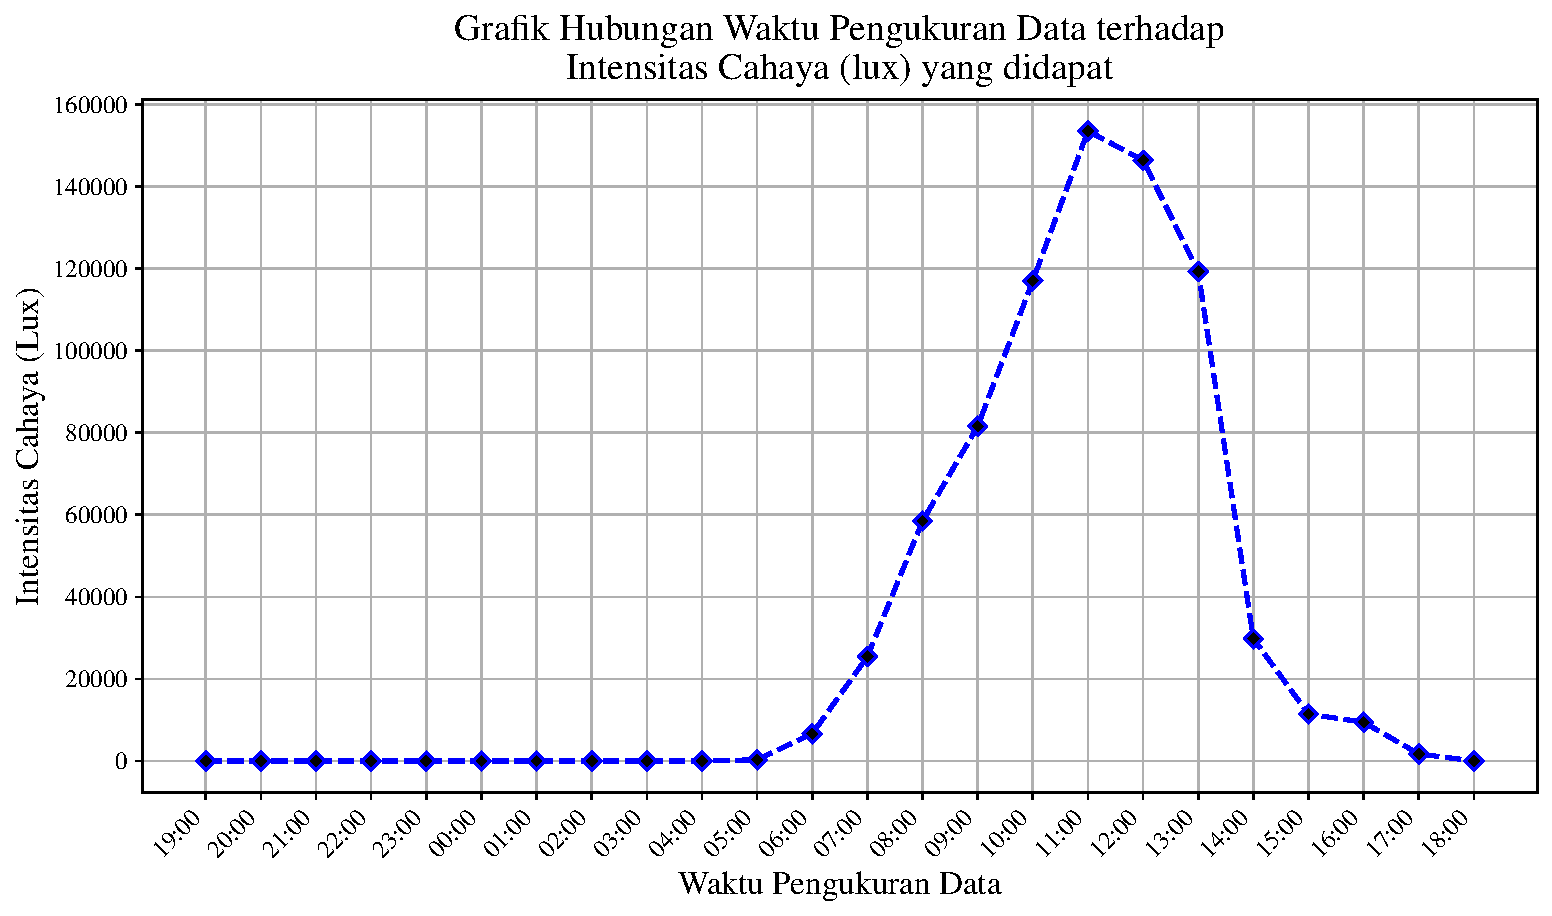
\includegraphics[width=0.95\textwidth]{dataset/grafik waktu vs intensitas.pdf}
    \caption{Grafik waktu pengukuran terhadap hasil ukur intensitas cahaya matahari dengan aplikasi \textit{Pengukur Cahaya}}
    \labfig{waktu-vs-intensitas}
\end{figure}
Berdasarkan \reffig{waktu-vs-intensitas}, intensitas cahaya matahari bervariasi. Pada fase malam hari ke dini hari mulai pukul 18.00 s.d. 04.00 intensitas cahaya matahari adalah 0. Sedangkan mulai pukul 05.00 cahaya matahari mulai terukur dan terus meningkat sampai pada puncaknya dengan rata-rata sebesar 153.540 Lux (pukul 11.00), kemudian mulai menurun kembali sampai nilai terendah pada pukul 17.00. Berdasarkan \reffig{waktu-vs-intensitas} dapat diketahui bahwa waktu tengah hari adalah sekitar pukul 11.00 atau antara 11.00 dan 12.00.

\subsection{Intensitas Cahaya Matahari Terhadap Suhu Udara}
\begin{figure}
    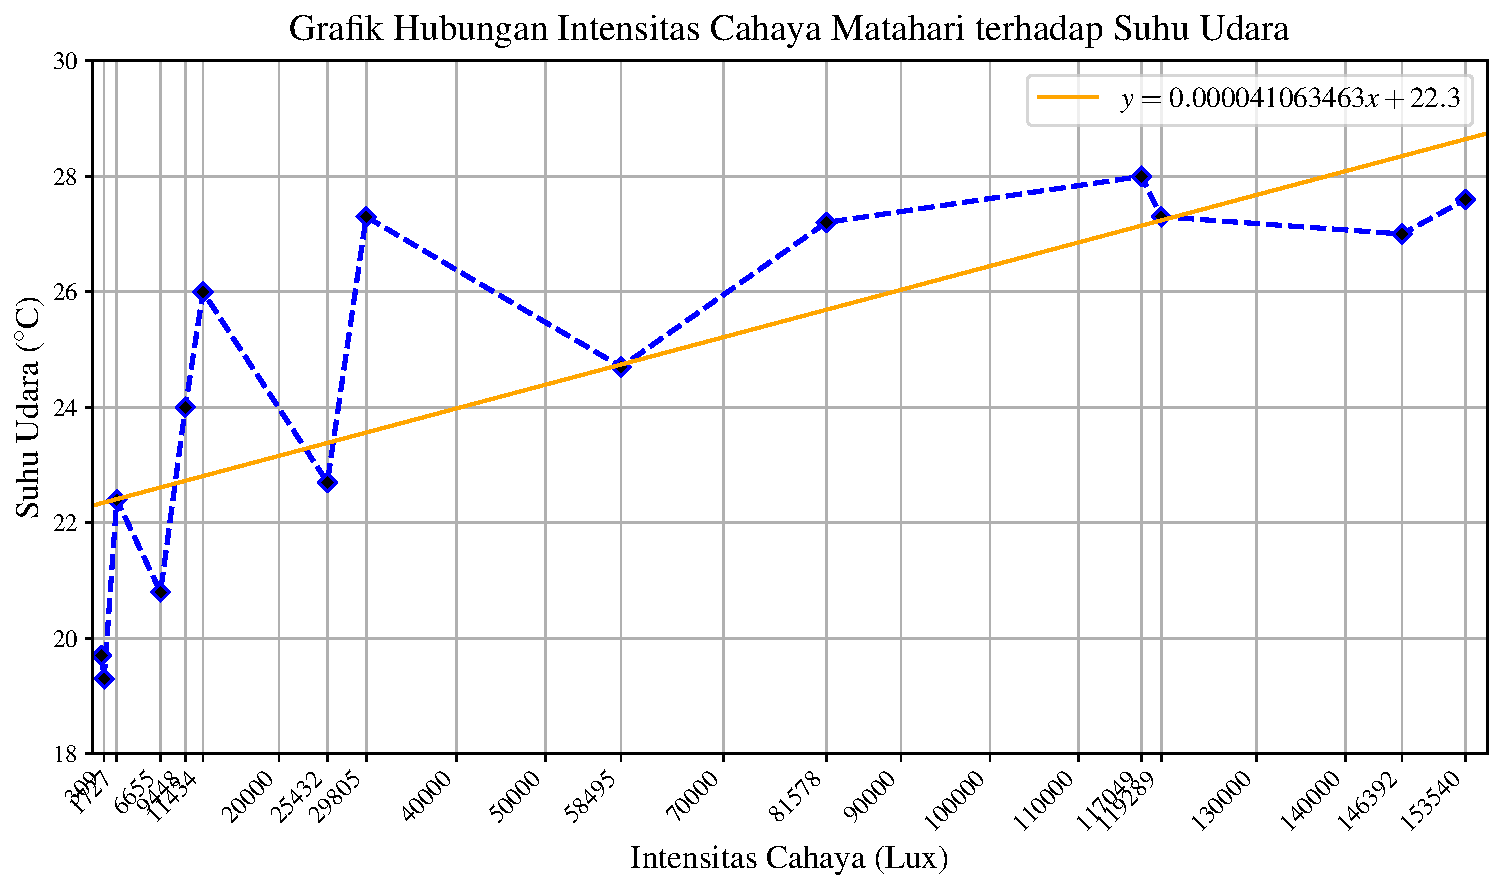
\includegraphics[width=0.95\textwidth]{dataset/grafik intensitas vs suhu.pdf}
    \caption{Grafik intensitas cahaya matahari terhadap suhu udara}
    \labfig{intensitas-vs-suhu}
\end{figure}
Berdasarkan \reffig{intensitas-vs-suhu} diperoleh suhu udara minimum yakni $19,3^\circ$ pada intensitas cahaya matahari 309,3 Lux. Data suhu minimum ini terukur pada pukul 05.00 WIB, Sabtu, 11 November 2023. Sedangkan suhu udara maksimum yakni $28,0^\circ$ pada intensitas cahaya matahari 117.049,3 Lux. Data suhu maksimum ini terukur pada pukul 10.00, Sabtu, 11 November 2023. Dari grafik intensitas cahaya matahari terhadap suhu udara terlihat tren suhu yang meningkat seiring pertambahan intensitas cahaya.

\subsection{Intensitas Cahaya Matahari Terhadap Kelembapan Udara}
\begin{figure}[H]
    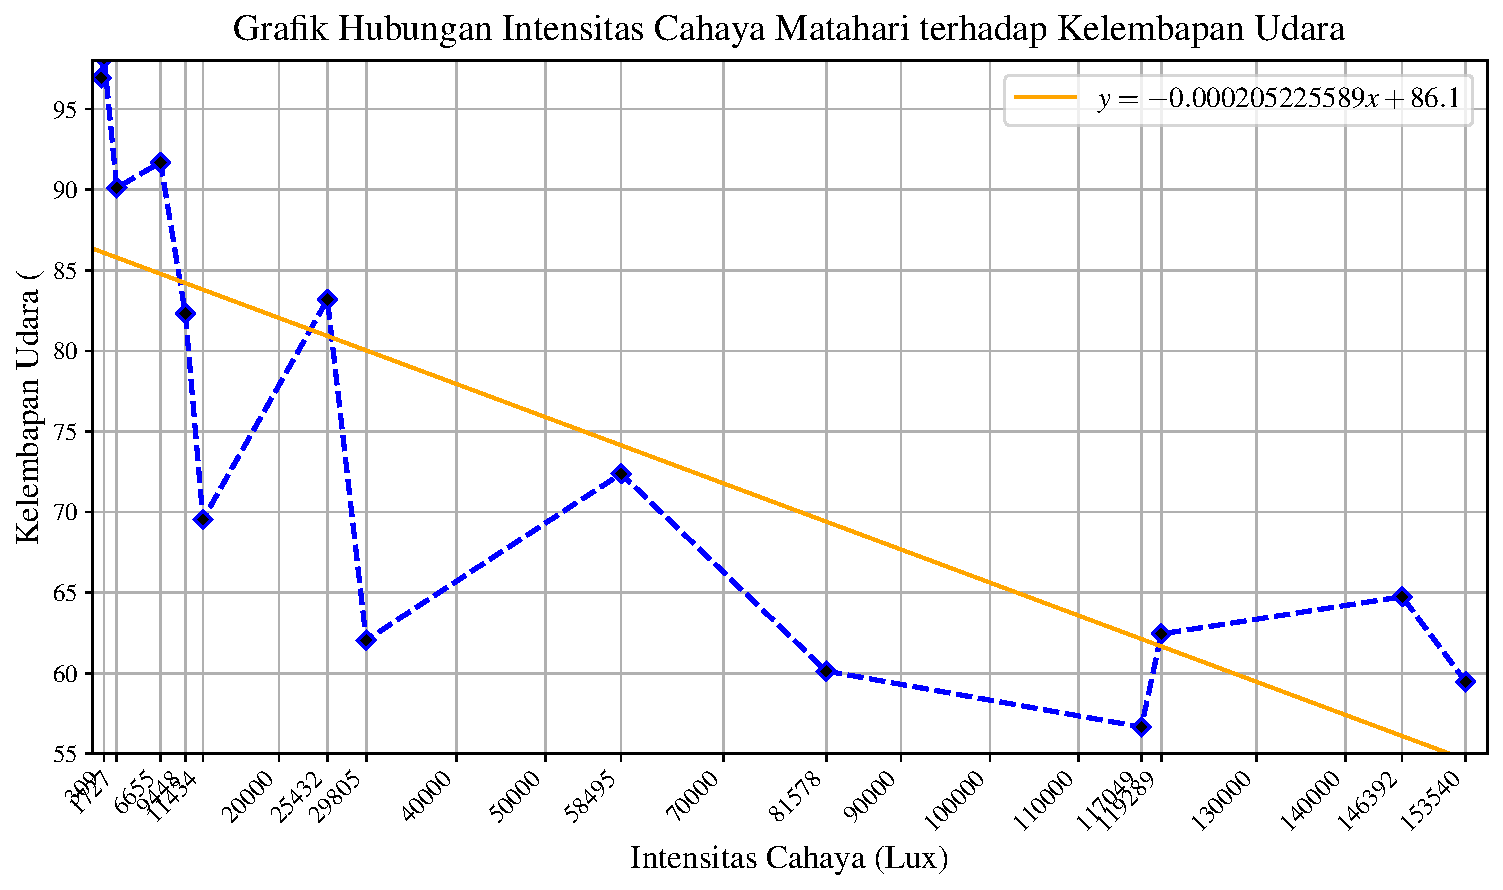
\includegraphics[width=0.95\textwidth]{dataset/grafik intensitas vs kelembapan.pdf}
    \caption{Grafik Intensitas Cahaya Matahari Terhadap Kelembapan Udara}
    \labfig{intensitas-vs-kelembapan}
\end{figure}
Berdasarkan \reffig{intensitas-vs-kelembapan}, diperoleh nilai minimum 56,66\% pada intensitas cahaya matahari 117.049,3 Lux. Data kelembapan minmum ini terukur pada pukul 10.00, Sabtu, 11 November 2023. Sedangkan kelembapan udara maksimum sebesar 98,15\% pada pukul 05.00 WIB dengan intensitas cahaya matahari 309,3 Lux, Sabtu, 11 November 2023. Dari grafik intensitas cahaya matahari terhadap kelembapan udara terlihat tren kelembapan yang menurun seiring pertambahan intensitas cahaya.



% >>>>>>>>>>>>>>>>>>> CHAPTER 5 PEMBAHASAN
\chapter{Pembahasan}
\section{Hubungan Posisi Matahari Terhadap Hasil Ukur Intensitas Cahaya Matahari Tiap Waktu}
Berdasarkan analisis data dapat diketahui bahwa terdapat hubungan antara waktu pengambilan data/pengukuran terhadap hasil ukur intensitas cahaya matahari yang didapat. Cahaya matahari mulai tampak pada pukul 05.00 WIB dan intensitasnya terus meningkat hingga pukul 11.00 WIB. Setelah pukul 11.00 WIB intensitas cahaya matahari mulai menurun hingga titik terkecilnya pada pukul 17.00 WIB. Pada pukul 18.00 s.d. 04.00 tidak ada intensitas cahaya matahari yang dapat diukur.  Ketiga bagian waktu ini dapat kita kelompokkan kedalam kelompok pagi-siang (pukul 05.00 s.d. 11.00 WIB), siang-sore (pukul 11.00 s.d. 17.00), dan malam-pagi (pukul 18.00 s.d. 04.00). Perlu diingat bahwa pengukuran dimulai pada tanggal 10 November pukul 19.00 dan berakhir pada 11 November pukul 18.00, tetapi disini tanggal atau hari tidak begitu penting. Hal yang penting adalah bahwa data diambil secara berkesinambungan selama 24 jam. 

Pada kelompok pagi-siang, intensitas cahaya matahari mulai terukur dan meningkat. Hal ini karena posisi matahari telah berada pada altitude $\geq 0^\circ$, sehingga setidaknya sebagian dari matahari sudah tampak di ufuk/horizon dan pandaran cahayanya dapat terdeteksi oleh \textit{Pengukur Cahaya/Lux meter}. Selanjutnya intensitas cahaya matahari terus bertambah sampai titik pengukuran maksimum pada pukul 11.00 dengan intensitas $153.539,6$  Lux. Pada pukul 11.00 posisi matahari berada pada altitude $80,27^\circ$ yang mana adalah altitude maksimum dalam projek ini. Secara teori, tentu, puncak intensitas cahaya matahari akan terukur antara pukul 11.00 dan 12.00, saat altitude nya $90^\circ$.

Pada kelompok siang-sore, intensitas cahaya matahari menurun sampai dengan intensitas terendahnya pada pukul 17.00 WIB dengan intensitas 1.727 Lux. Penurunan intensitas cahaya matahari ini terjadi seiring dengan menurunnya altitude matahari. Pada pukul 17.00 WIB, di mana matahari terbenam, altitude matahari berada pada $5,54^\circ$. Pada pukul 17.00 WIB altitude matahari lebih besar dari $0^\circ$ sehingga jika dibandingkan dengan intensitas pada pagi hari pukul 5.00 WIB didapatkan hasil pengukuran yang lebih besar.

Pada kelompok malam-pagi, intensitas cahaya matahari tidak dapat diukur sama sekali. Hal ini mengakibatkan pembacaan Lux meter menjadi 0 Lux. Pada kelompok malam-pagi posisi matahari berada pada altitude negatif. Altitude negatif berarti bahwa matahari berada di bawah horizon pada waktu tertentu ditinjau dari suatu tempat, sehingga tidak ada intensitas cahaya matahari yang dapat terukur. Pada saat ini matahari mulai berpindah ke belahan lain dari Bumi sebagai akibat dari rotasi bumi sambil melakukan revolusi terhadap matahari. 

Dalam pembahasan pada tiga pengelompokan tersebut, perlu diingat bahwa hubungan antara posisi dan intensitas cahaya matahari tiap waktunya tidak dapat dimodelkan kedalam kesebandingan atau ketidaksebandingan linier. Di sini kita baru membahas, posisi matahari ditinjau dari altitude atau sudut ketinggiannya dari posisi pengukur. Terdapat dua data lain yang menjelaskan posisi matahari, yakni sudut azimuth dan deklinasi. Ketiga data posisi (altitude, azimuth, dan deklinasi) ini dapat dianalisis lebih lanjut untuk menentukan lintasan matahari pada tiap waktu, hari, bulan, maupun tahun. Namun, hal ini akan melibatkan perhitungan dan tinjauan geometri yang kompleks.

Selain posisi, sebenarnya tedapat faktor-faktor lain yang dapat mempengaruhi hasil pengukuran intensitas cahaya matahari. Cahaya matahari yang melewati atmosfer dengan berbagai macam partikel akan mengalami hamburan dan serapan. Serapann dan hamburan, seperti hamburan Rayleigh, Mie, dan non selektif mempengaruhi rentang panjang gelombang yang sampai pada pengukur. Panjang gelombang cahaya yang datang kepada pengukur tentu mempengaruhi pembacaan intensitas terukur. Selain itu jika terjadi hamburan non selektif akibat sekumpulan awan hujan yang tebal, tentu akan mengurangi intensitas cahaya matahari yang terukur oleh Lux Meter.

\section{Hubungan Intensitas Cahaya Matahari Terhadap Suhu Udara}
Pada bagian ini data juga diurutkan mulai dari intensitas cahaya matahari terkecil, yakni 0 Lux sampai dengan intensitas cahaya terbesar 153.539,6 Lux. Untuk menjaga kontinuitas data, untuk intensitas cahaya matahari terkecil (0 Lux), dari data pukul 18.00 s.d. 04.00, diambil data pada pukul 04.00 WIB. Sedangkang untuk intensitas cahaya matahari terbesar terdapat pada data pukul 11.00 WIB. Data intensitas cahaya matahari dan suhu udara tiap waktu ini kemudian di plot dalam garfik sebaran dengan analisis regresi linier.

Berdaskan analisis data, suhu udara menunjukkan tren yang berbanding lurus dengan intensitas cahaya matahari. Suhu udara minimum terukur sebesar $19,3^\circ$ pada intensitas cahaya matahari 309,3 Lux. Data suhu minimum ini terukur pada pukul 05.00 WIB. Sedangkan suhu udara maksimum yakni $28,0^\circ$ pada intensitas cahaya matahari 117.049,3 Lux. Data suhu maksimum ini terukur pada pukul 10.00. 

Seluruh energi dari matahari, sampai ke Bumi dalam bentuk radiasi matahari, sebagai bagian dari sekumpulan energi yang disebut spektrum radiasi elektromagnetik. Radiasi matahari memuat cahaya tampak, cahaya ultraviolet, infrared, radio, sinar-X, dan sinar Gamma. Radiasi ini merupakan salah satu cara untuk mendistribusikan panas. Inilah yang mengakibatkan intensitas cahaya matahari berpengaruh terhadap suhu udara yang dilewatinya.

\section{Hubungan Intensitas Cahaya Matahari Terhadap Kelembapan Udara}
Pada bagian ini data juga diurutkan mulai dari intensitas cahaya matahari terkecil, yakni 0 Lux sampai dengan intensitas cahaya terbesar 153.539,6 Lux. Untuk menjaga kontinuitas data, untuk intensitas cahaya matahari terkecil (0 Lux), dari data pukul 18.00 s.d. 04.00, diambil data pada pukul 04.00 WIB. Sedangkang untuk intensitas cahaya matahari terbesar terdapat pada data pukul 11.00 WIB. Data intensitas cahaya matahari dan kelembapan udara tiap waktu ini kemudian di plot dalam garfik sebaran dengan analisis regresi linier.

Suhu udara, tentu berbanding terbalik dengan kelembapan udara. Seiring dengan pertambahan panas udara maka udara akan mengering karena jumlah uap air yang berkurang. Dari sini dapat dikatahui bahwa hubungan antara intensitas cahaya matahari yang sebanding dengan suhu pasti akan berbanding terbalik dengan kelembapan udara. Dapat dilihat pada bagian analisis data, nilai minimum kelembapan udara, yakni 56,66\% pada intensitas cahaya matahari 117.049,3 Lux. Sedangkan kelembapan udara maksimum sebesar 98,15\% pada intensitas cahaya matahari 309,3 Lux.

% >>>>>>>>>>>>>>>>>>> CHAPTER 6 KESIMPULAN DAN PENUTUP
\chapter{Penutup}
\section{Kesimpulan}
Kesimpulan dari percobaan yang dilakukan adalah,
\begin{enumerate}[leftmargin=*]
    \item Hubungan antara waktu pengukuran terhadap hasil ukur intensitas cahaya matahari menggunakan Lux Meter adalah berbanding lurus untuk kelompok waktu pagi ke siang, berbanding terbalik untuk kelompok waktu siang ke malam, dan nol pada waktu malam hingga dini hari.
    \item Posisi matahari, dalam hal ini altitude, berhubungan dengan intensitas cahaya matahari yang terkur dengan tren berbanding lurus.
    \item Suhu udara berbanding lurus dengan intensitas cahaya matahari yang datang.
    \item Kelembapan udara berbanding terbalik dengan intensitas cahaya matahari yang datang.
\end{enumerate}

\section{Saran}
Selanjutnya dapat dilakukan kajian yang lebih spesifik dan tidak terbatas hanya pada hubungan antara intensitas cahaya matahari dengan posisi, suhu udara, dan kelembapan udara tiap waktunya secara umum. Sebelum melakukan percobaan maka peneliti perlu memahami dengan baik variabel-variabel apa yang akan diukur dan variabel apa yang pengaruhnya akan dikontrol. Dalam hal alat ukur, dapat digunakan alat ukur khusus untuk pengukuran intensitas cahaya matahari, sehingga hasil pengukuran tidak lagi bergantung terhadap kualitas sensor cahaya dari \textit{smartphone} yang memang telah disesuaikan untuk kebutuhan tertentu.


\bibliographystyle{ieeetr}
\bibliography{referensi}

% >>>>>>>>>>>>>>>>>>> CHAPTER KESIMPULAN DAN PENUTUP
\chapter{Lampiran}
\section{Data Pengukuran Intensitas Cahaya Matahari}
\begin{widepage}
\begin{center}
\begin{longtable}{|p{0.9cm}| C{4.2cm} | C{4.2cm} | C{4.2cm}|}
    \hline
    \rowcolor[rgb]{0.961,0.961,0.961} \textbf{Jam} & \textbf{Data 1} & \textbf{Data 2} & \textbf{Data 3} \\
    \hhline{----}
19:00 & \adjustbox{valign=t}{\includegraphics[width=4.1cm]{gambar/Screenshots/19a.jpg}} & \adjustbox{valign=t}{\includegraphics[width=4.1cm]{gambar/Screenshots/19b.jpg}}   & \adjustbox{valign=t}{\includegraphics[width=4.1cm]{gambar/Screenshots/19c.jpg}}\\\hline
20:00 & \adjustbox{valign=t}{\includegraphics[width=4.1cm]{gambar/Screenshots/20a.jpg}} & \adjustbox{valign=t}{\includegraphics[width=4.1cm]{gambar/Screenshots/20b.jpg}}   & \adjustbox{valign=t}{\includegraphics[width=4.1cm]{gambar/Screenshots/20c.jpg}}\\\hline
21:00 & \adjustbox{valign=t}{\includegraphics[width=4.1cm]{gambar/Screenshots/21a.jpg}} & \adjustbox{valign=t}{\includegraphics[width=4.1cm]{gambar/Screenshots/21b.jpg}}   & \adjustbox{valign=t}{\includegraphics[width=4.1cm]{gambar/Screenshots/21c.jpg}}\\\hline
22:00 & \adjustbox{valign=t}{\includegraphics[width=4.1cm]{gambar/Screenshots/22a.jpg}} & \adjustbox{valign=t}{\includegraphics[width=4.1cm]{gambar/Screenshots/22b.jpg}}   & \adjustbox{valign=t}{\includegraphics[width=4.1cm]{gambar/Screenshots/22c.jpg}}\\\hline
23:00 & \adjustbox{valign=t}{\includegraphics[width=4.1cm]{gambar/Screenshots/23a.jpg}} & \adjustbox{valign=t}{\includegraphics[width=4.1cm]{gambar/Screenshots/23b.jpg}}   & \adjustbox{valign=t}{\includegraphics[width=4.1cm]{gambar/Screenshots/23c.jpg}}\\\hline
00:00 & \adjustbox{valign=t}{\includegraphics[width=4.1cm]{gambar/Screenshots/00a.jpg}} & \adjustbox{valign=t}{\includegraphics[width=4.1cm]{gambar/Screenshots/00b.jpg}}   & \adjustbox{valign=t}{\includegraphics[width=4.1cm]{gambar/Screenshots/00c.jpg}}\\\hline
01:00 & \adjustbox{valign=t}{\includegraphics[width=4.1cm]{gambar/Screenshots/1a.jpg}}  & \adjustbox{valign=t}{\includegraphics[width=4.1cm]{gambar/Screenshots/1b.jpg}}    & \adjustbox{valign=t}{\includegraphics[width=4.1cm]{gambar/Screenshots/1c.jpg}}\\\hline
02:00 & \adjustbox{valign=t}{\includegraphics[width=4.1cm]{gambar/Screenshots/2a.jpg}}  & \adjustbox{valign=t}{\includegraphics[width=4.1cm]{gambar/Screenshots/2b.jpg}}    & \adjustbox{valign=t}{\includegraphics[width=4.1cm]{gambar/Screenshots/2c.jpg}}\\\hline
03:00 & \adjustbox{valign=t}{\includegraphics[width=4.1cm]{gambar/Screenshots/3a.jpg}}  & \adjustbox{valign=t}{\includegraphics[width=4.1cm]{gambar/Screenshots/3b.jpg}}    & \adjustbox{valign=t}{\includegraphics[width=4.1cm]{gambar/Screenshots/3c.jpg}}\\\hline
04:00 & \adjustbox{valign=t}{\includegraphics[width=4.1cm]{gambar/Screenshots/4a.jpg}}  & \adjustbox{valign=t}{\includegraphics[width=4.1cm]{gambar/Screenshots/4b.jpg}}    & \adjustbox{valign=t}{\includegraphics[width=4.1cm]{gambar/Screenshots/4c.jpg}}\\\hline
05:00 & \adjustbox{valign=t}{\includegraphics[width=4.1cm]{gambar/Screenshots/5a.jpg}}  & \adjustbox{valign=t}{\includegraphics[width=4.1cm]{gambar/Screenshots/5b.jpg}}    & \adjustbox{valign=t}{\includegraphics[width=4.1cm]{gambar/Screenshots/5c.jpg}}\\\hline
06:00 & \adjustbox{valign=t}{\includegraphics[width=4.1cm]{gambar/Screenshots/6a.jpg}}  & \adjustbox{valign=t}{\includegraphics[width=4.1cm]{gambar/Screenshots/6b.jpg}}    & \adjustbox{valign=t}{\includegraphics[width=4.1cm]{gambar/Screenshots/6c.jpg}}\\\hline
07:00 & \adjustbox{valign=t}{\includegraphics[width=4.1cm]{gambar/Screenshots/7a.jpg}}  & \adjustbox{valign=t}{\includegraphics[width=4.1cm]{gambar/Screenshots/7b.jpg}}    & \adjustbox{valign=t}{\includegraphics[width=4.1cm]{gambar/Screenshots/7c.jpg}}\\\hline
08:00 & \adjustbox{valign=t}{\includegraphics[width=4.1cm]{gambar/Screenshots/8a.jpg}}  & \adjustbox{valign=t}{\includegraphics[width=4.1cm]{gambar/Screenshots/8b.jpg}}    & \adjustbox{valign=t}{\includegraphics[width=4.1cm]{gambar/Screenshots/8c.jpg}}\\\hline
09:00 & \adjustbox{valign=t}{\includegraphics[width=4.1cm]{gambar/Screenshots/9a.jpg}}  & \adjustbox{valign=t}{\includegraphics[width=4.1cm]{gambar/Screenshots/9b.jpg}}    & \adjustbox{valign=t}{\includegraphics[width=4.1cm]{gambar/Screenshots/9c.jpg}}\\\hline
10:00 & \adjustbox{valign=t}{\includegraphics[width=4.1cm]{gambar/Screenshots/10a.jpg}} & \adjustbox{valign=t}{\includegraphics[width=4.1cm]{gambar/Screenshots/10b.jpg}}   & \adjustbox{valign=t}{\includegraphics[width=4.1cm]{gambar/Screenshots/10c.jpg}}\\\hline
11:00 & \adjustbox{valign=t}{\includegraphics[width=4.1cm]{gambar/Screenshots/11a.jpg}} & \adjustbox{valign=t}{\includegraphics[width=4.1cm]{gambar/Screenshots/11b.jpg}}   & \adjustbox{valign=t}{\includegraphics[width=4.1cm]{gambar/Screenshots/11c.jpg}}\\\hline
12:00 & \adjustbox{valign=t}{\includegraphics[width=4.1cm]{gambar/Screenshots/12a.jpg}} & \adjustbox{valign=t}{\includegraphics[width=4.1cm]{gambar/Screenshots/12b.jpg}}   & \adjustbox{valign=t}{\includegraphics[width=4.1cm]{gambar/Screenshots/12c.jpg}}\\\hline
13:00 & \adjustbox{valign=t}{\includegraphics[width=4.1cm]{gambar/Screenshots/13a.jpg}} & \adjustbox{valign=t}{\includegraphics[width=4.1cm]{gambar/Screenshots/13b.jpg}}   & \adjustbox{valign=t}{\includegraphics[width=4.1cm]{gambar/Screenshots/13c.jpg}}\\\hline
14:00 & \adjustbox{valign=t}{\includegraphics[width=4.1cm]{gambar/Screenshots/14a.jpg}} & \adjustbox{valign=t}{\includegraphics[width=4.1cm]{gambar/Screenshots/14b.jpg}}   & \adjustbox{valign=t}{\includegraphics[width=4.1cm]{gambar/Screenshots/14c.jpg}}\\\hline
15:00 & \adjustbox{valign=t}{\includegraphics[width=4.1cm]{gambar/Screenshots/15a.jpg}} & \adjustbox{valign=t}{\includegraphics[width=4.1cm]{gambar/Screenshots/15b.jpg}}   & \adjustbox{valign=t}{\includegraphics[width=4.1cm]{gambar/Screenshots/15c.jpg}}\\\hline
16:00 & \adjustbox{valign=t}{\includegraphics[width=4.1cm]{gambar/Screenshots/16a.jpg}} & \adjustbox{valign=t}{\includegraphics[width=4.1cm]{gambar/Screenshots/16b.jpg}}   & \adjustbox{valign=t}{\includegraphics[width=4.1cm]{gambar/Screenshots/16c.jpg}}\\\hline
17:00 & \adjustbox{valign=t}{\includegraphics[width=4.1cm]{gambar/Screenshots/17a.jpg}} & \adjustbox{valign=t}{\includegraphics[width=4.1cm]{gambar/Screenshots/17b.jpg}}   & \adjustbox{valign=t}{\includegraphics[width=4.1cm]{gambar/Screenshots/17c.jpg}}\\\hline
18:00 & \adjustbox{valign=t}{\includegraphics[width=4.1cm]{gambar/Screenshots/18a.jpg}} & \adjustbox{valign=t}{\includegraphics[width=4.1cm]{gambar/Screenshots/18b.jpg}}   & \adjustbox{valign=t}{\includegraphics[width=4.1cm]{gambar/Screenshots/18c.jpg}}\\\hline
\caption{Dokumentasi Data Pengukuran Intensitas Cahaya Matahari}
\labtab{dokumentasi1}
\end{longtable}
\end{center}
\end{widepage}

\section{Intensitas Cahaya Matahari, Posisi Matahari, Cuaca, Analisis Data}
Data intensitas cahaya matahari, posisi matahari, cuaca, dan analisisnya dapat diunduh pada \href{https://github.com/firman-qs/Firmanqs-Proyek-Optika-Intensitas-Cahaya/blob/main/data.ipynb}{notebook berikut}.

\section{Dokumentasi Pengukuran Intensitas Cahaya Matahari}
\begin{longtable}[l]{|p{0.9cm}| C{4.2cm} |}
    \hline
    \rowcolor[rgb]{0.961,0.961,0.961} \textbf{Jam} & \textbf{Dokumentasi} \\
    \hhline{--}
19:00 & \adjustbox{valign=t}{\includegraphics[width=4.1cm]{gambar/Dokumentasi_pengambilan_data/19.jpg}} \\\hline
20:00 & \adjustbox{valign=t}{\includegraphics[width=4.1cm]{gambar/Dokumentasi_pengambilan_data/20.jpg}} \\\hline
21:00 & \adjustbox{valign=t}{\includegraphics[width=4.1cm]{gambar/Dokumentasi_pengambilan_data/21.jpg}} \\\hline
22:00 & \adjustbox{valign=t}{\includegraphics[width=4.1cm]{gambar/Dokumentasi_pengambilan_data/22.jpg}} \\\hline
23:00 & \adjustbox{valign=t}{\includegraphics[width=4.1cm]{gambar/Dokumentasi_pengambilan_data/23.jpg}} \\\hline
00:00 & \adjustbox{valign=t}{\includegraphics[width=4.1cm]{gambar/Dokumentasi_pengambilan_data/00.jpg}} \\\hline
01:00 & \adjustbox{valign=t}{\includegraphics[width=4.1cm]{gambar/Dokumentasi_pengambilan_data/IMG-20231110-WA0013.jpg}}  \\\hline
02:00 & \adjustbox{valign=t}{\includegraphics[width=4.1cm]{gambar/Dokumentasi_pengambilan_data/2.jpg}}  \\\hline
03:00 & \adjustbox{valign=t}{\includegraphics[width=4.1cm]{gambar/Dokumentasi_pengambilan_data/3.jpg}}  \\\hline
04:00 & \adjustbox{valign=t}{\includegraphics[width=4.1cm]{gambar/Dokumentasi_pengambilan_data/4.jpg}}  \\\hline
05:00 & \adjustbox{valign=t}{\includegraphics[width=4.1cm]{gambar/Dokumentasi_pengambilan_data/5.jpg}}  \\\hline
06:00 & \adjustbox{valign=t}{\textit{Tidak terdokumentasi}}  \\\hline
07:00 & \adjustbox{valign=t}{\includegraphics[width=4.1cm]{gambar/Dokumentasi_pengambilan_data/7.jpg}}  \\\hline
08:00 & \adjustbox{valign=t}{\includegraphics[width=4.1cm]{gambar/Dokumentasi_pengambilan_data/8.jpg}}  \\\hline
09:00 & \adjustbox{valign=t}{\includegraphics[width=4.1cm]{gambar/Dokumentasi_pengambilan_data/9.jpg}}  \\\hline
10:00 & \adjustbox{valign=t}{\includegraphics[width=4.1cm]{gambar/Dokumentasi_pengambilan_data/10.jpg}} \\\hline
11:00 & \adjustbox{valign=t}{\includegraphics[width=4.1cm]{gambar/Dokumentasi_pengambilan_data/11.jpg}} \\\hline
12:00 & \adjustbox{valign=t}{\includegraphics[width=4.1cm]{gambar/Dokumentasi_pengambilan_data/12.jpg}} \\\hline
13:00 & \adjustbox{valign=t}{\includegraphics[width=4.1cm]{gambar/Dokumentasi_pengambilan_data/13.jpg}} \\\hline
14:00 & \adjustbox{valign=t}{\includegraphics[width=4.1cm]{gambar/Dokumentasi_pengambilan_data/14.jpg}} \\\hline
15:00 & \adjustbox{valign=t}{\textit{Tidak terdokumentasi}} \\\hline
16:00 & \adjustbox{valign=t}{\textit{Tidak terdokumentasi}} \\\hline
17:00 & \adjustbox{valign=t}{\textit{Tidak terdokumentasi}} \\\hline
18:00 & \adjustbox{valign=t}{\textit{Tidak terdokumentasi}} \\\hline
\caption{Dokumentasi Pengukuran Intensitas Cahaya Matahari}
\labtab{dokumentasi1}
\end{longtable}

\end{document}
